\documentclass[twocolumn,a4j]{jsarticle}
\bibliographystyle{junsrt}

\setlength{\topmargin}{-20.4cm}
\setlength{\oddsidemargin}{-10.4mm}
\setlength{\evensidemargin}{-10.4mm}
\setlength{\textwidth}{18cm}
\setlength{\textheight}{26cm}

\usepackage[top=15truemm,bottom=20truemm,left=20truemm,right=20truemm]{geometry}
\usepackage[latin1]{inputenc}
\usepackage{amsmath}
\usepackage{amsfonts}
\usepackage{amssymb}
\usepackage[dvipdfmx]{graphicx}
\usepackage[hang,small,bf]{caption}
\usepackage[subrefformat=parens]{subcaption}
\usepackage[dvipdfmx]{color}
\usepackage{listings}
\usepackage{listings,jvlisting}
\usepackage{geometry}
\usepackage{framed}
\usepackage{color}
\usepackage[dvipdfmx]{hyperref}
\usepackage{ascmac}
\usepackage{enumerate}
\usepackage{tabularx}
\usepackage{cancel}
\usepackage{scalefnt}
\usepackage{overcite}
\usepackage{otf}

\renewcommand{\figurename}{Fig.}
\renewcommand{\tablename}{Table }

\hypersetup{%
    hidelinks %リンクの色消し
}

\lstset{
basicstyle={\ttfamily},
identifierstyle={\small},
commentstyle={\smallitshape},
keywordstyle={\small\bfseries},
ndkeywordstyle={\small},
stringstyle={\small\ttfamily},
frame={tb},
breaklines=true,
columns=[l]{fullflexible},
xrightmargin=0zw,
xleftmargin=3zw,
numberstyle={\scriptsize},
stepnumber=1,
numbersep=1zw,
lineskip=-0.5ex
}

% キャプション後ろのダブルコロンを消す
\makeatletter
\long\def\@makecaption#1#2{%
  \vskip\abovecaptionskip
  \iftdir\sbox\@tempboxa{#1\hskip1zw#2}%
    \else\sbox\@tempboxa{#1 #2}%
  \fi
  \ifdim \wd\@tempboxa >\hsize
    \iftdir #1\hskip1zw#2\relax\par
      \else #1 #2\relax\par\fi
  \else
    \global \@minipagefalse
    \hbox to\hsize{\hfil\box\@tempboxa\hfil}%
  \fi
  \vskip\belowcaptionskip}
\makeatother


\makeatletter
\def\@maketitle
{
\begin{center}
{\LARGE \@title \par}
\end{center}
\begin{flushright}
{\large \@date}\\
{\large M2 \@author}
\end{flushright}
\par\vskip 1.5em
}
\makeatother

\author{来代 勝胤 / KITADAI Masatsugu}
\title{令和5年度 5月度 月例報告書}
\date{2023/05/30}

\begin{document}
\columnseprule=0.1mm
\maketitle

\section*{報告内容}
\begin{enumerate}[1.]
  \item 研究概要
  \item 三角翼後流の計測
  \item 車両モデル周りの流れ計測
  \item 6月の予定
\end{enumerate}

\section*{進捗報告}
今月は,可視化情報シンポジウムの原稿作成に向けた
三角翼後流と車両モデル周りにおける二次流れの計測実験を行った.

\section{研究概要}
輸送機械の設計および開発を行うにあたり,流体による作用力の影響を考慮しなければならない.
特に進行を妨げる方向にはたらく抗力の低減は,輸送機械の燃費向上を考える上で非常に重要だといえる.
また,その抗力の原因となる要素の一つとして,揚力の発生に伴う誘導抵抗が挙げられる.
航空機の亜音速飛行時には,全抵抗30~40\%を誘導抵抗が占めるとされており,
翼の吹きおろしに伴って縦渦が発生する.
また,自動車のルーフ後方に渦流発生器を取り付け,
意図的に縦渦を発生させることで流れの剥離を抑制する効果があることがわかっている.
したがって,輸送機械の設計・開発において抗力を考慮する際には,
機体周りの流れ場および主流方向に垂直な面内の二次流れ構造の理解が必要不可欠であるといえる.
そこで,二次流れ構造を定量的に評価するための計測手法の開発を目的に研究を行う.

\section{三角翼後流の計測}

\subsection{計測位置について}
今回は,Fig.1に示す三角翼モデルの後流について
Fig.2のように設置し,後方50mmの位置を対象として計測を行った.
また,撮影条件は以下の Table 1 の通りである.

\begin{table}[h]
  \label{table:data_type}
  \centering
  \caption{Experimental conditions}
  \begin{tabular}{| l | r | l |}
    \hline
    Mainstream velocity   & 250              & [mm/s]  \\ \hline
    Laser sheets distance & 2.5              & [mm]    \\ \hline
    Image size            & 800 $\times$ 600 & [px]    \\ \hline
    Frame rate            & 800              & [fps]   \\ \hline
    Shutter Speed         & 1/1000           & [s]     \\ \hline
    number of shots       & 4000             & [sheet] \\ \hline
  \end{tabular}
\end{table}

\begin{figure}[htbp]
  \footnotesize
  \begin{center}
    \includegraphics[width=50mm]{../images/delta_wing_model.jpg}
    \caption{Delta wing model}
    \includegraphics[width=60mm]{../images/delta_wing_position.png}
    \caption{Measurement position of delta wing wake}
  \end{center}
\end{figure}

\newpage

\subsection{解析結果}
Fig.3 にPTVの時間平均結果を示す.
結果より,$(y,z) = (50, 15)$を中心として反時計回りの渦の発生を見ることができる.
一方で渦の左側が鮮明に解析されていることに対して,右側は形が崩れていることもわかる.
これは,斜め後方からの撮影によって,カメラ手前側に当たる左側の情報量が大きく
奥側に当たる右側の情報量が少ない影響であると考える.

\begin{figure}[htbp]
  \footnotesize
  \begin{center}
    \includegraphics[width=85mm]{../images/time-averaged_velosity_of_delta_wake.png}
    \caption{Time-averaged velocity for wake of delta}
  \end{center}
\end{figure}

\newpage

\section{車両モデル周りの流れ計測}

\subsection{車両モデルの設置}
続いて,車両モデルを用いた流れの計測を行うにあたり,
回流水槽にFig.4 に示すようにタイヤモデル及び車体モデルを取り付け
設置した.また,タイヤモデルは主流速度に対応して回転させることができる.
一方,地面板については以前使用していたものを使用しているため,
再度撥水加工を行う予定である.

\begin{figure}[htbp]
  \footnotesize
  \begin{center}
    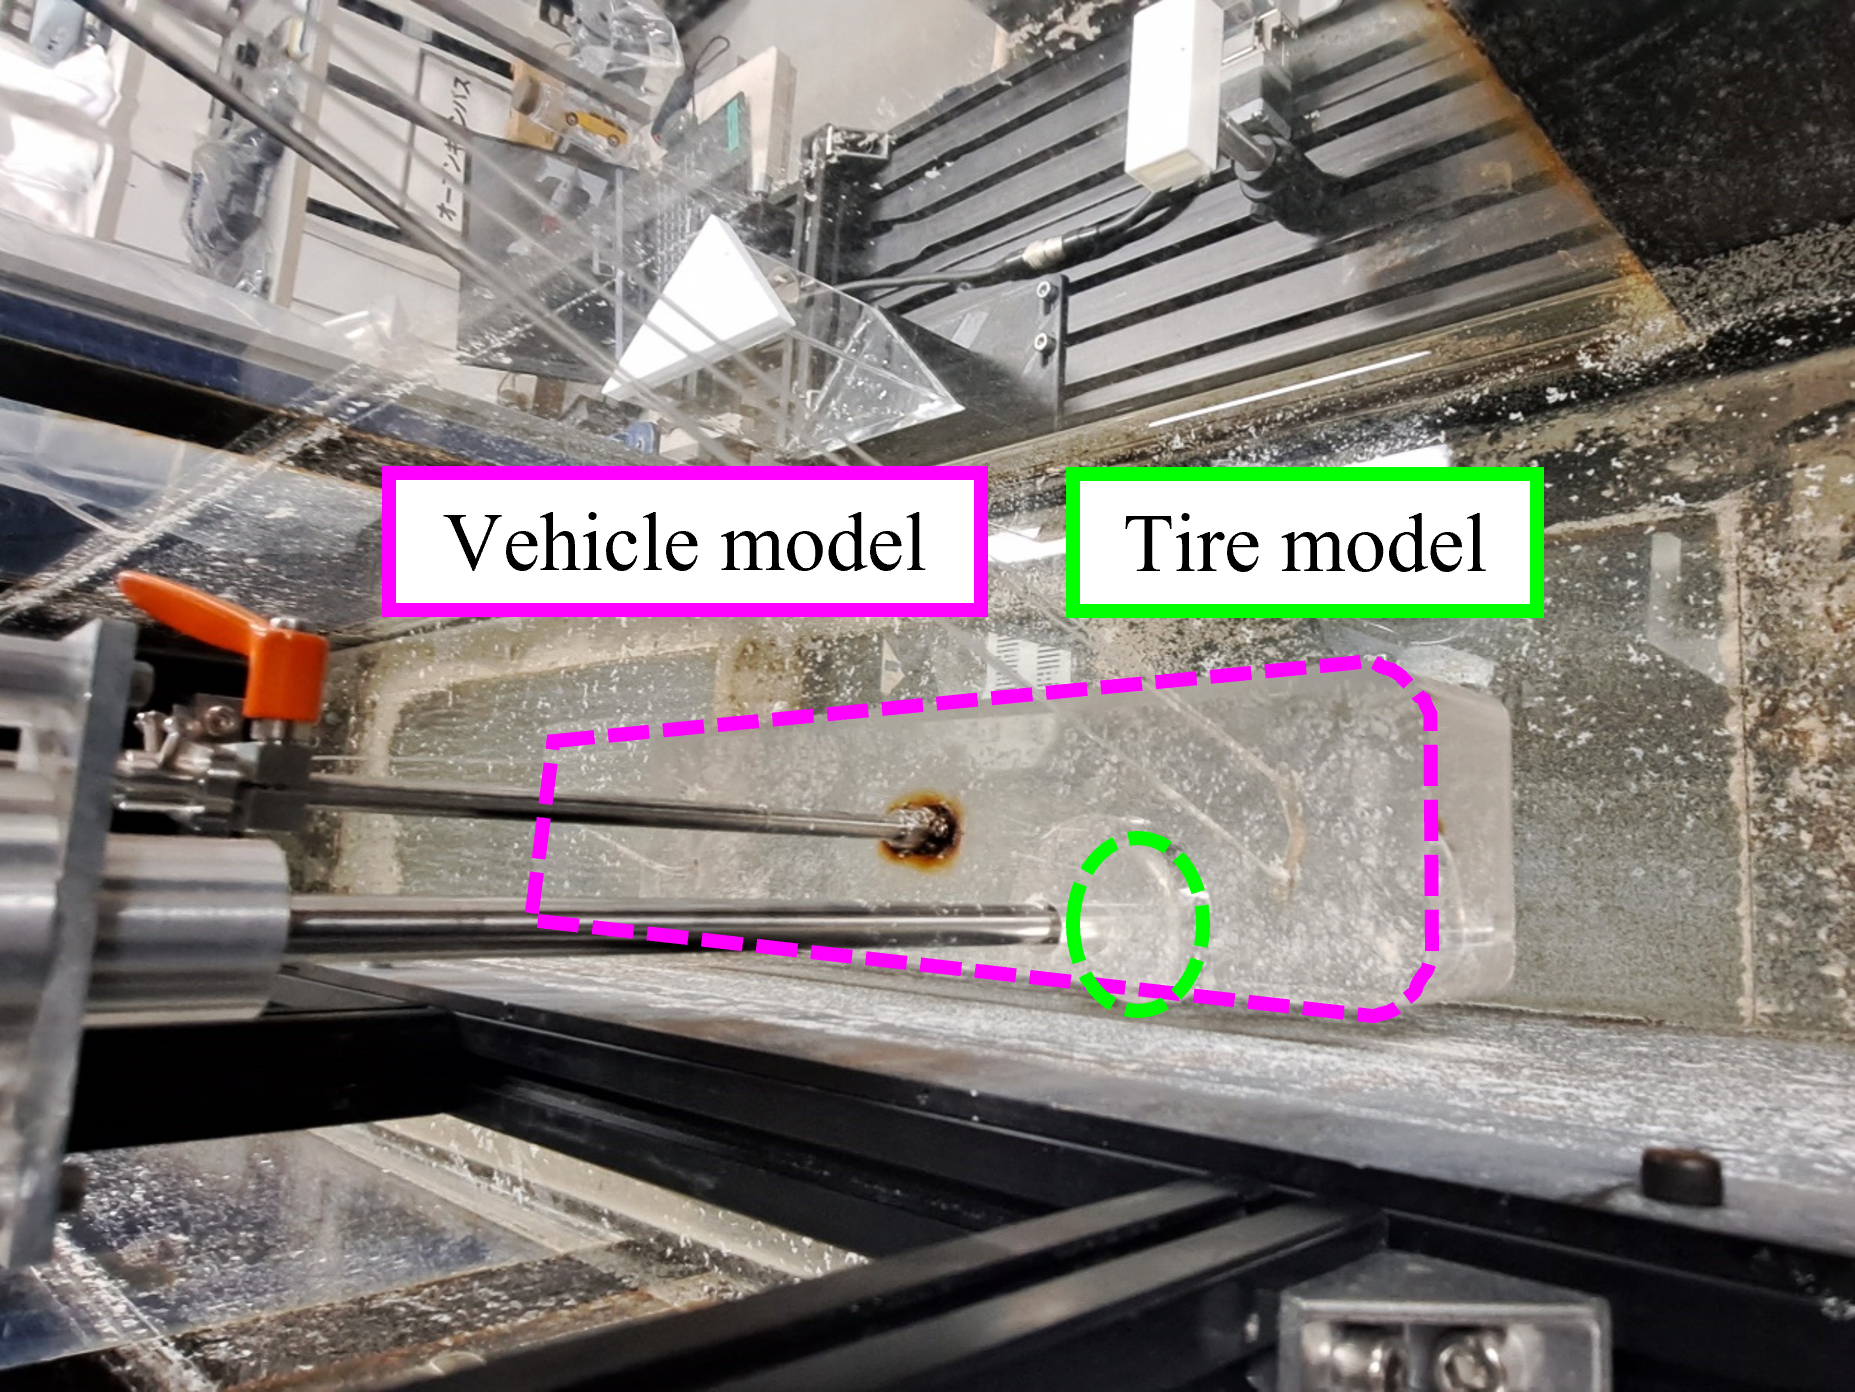
\includegraphics[width=60mm]{../images/vehicle_model.png}
    \caption{Vehicle model}
  \end{center}
\end{figure}

\subsection*{計測位置について}
今回の計測は,Fig.5に示すようにLLSを設置し,
車両モデルのタイヤ車軸から後方50mmの位置を撮影した.
なお,撮影は三角翼後流と同様に
Table 1 に示す条件で行った.

\begin{figure}[htbp]
  \footnotesize
  \begin{center}
    \includegraphics[width=50mm]{../images/experiment.jpg}
    \caption{Measurement position of wheelhouse wake}
  \end{center}
\end{figure}

\newpage
\subsection*{解析結果}
Fig.6にPTVの時間平均結果を示す.
結果の上部にタイヤモデルが設置されているためベクトルの表示はない.
結果をみると,三角翼のように定常的な流れの発生ではないことから
時間平均の流れ場に定常性はないことが確認できる.
車両モデルの二次流れの撮影は達成したが,
データの解析方法及び撮影条件については今後検討する必要がある.

\begin{figure}[htbp]
  \footnotesize
  \begin{center}
    \includegraphics[width=70mm]{../images/time-averaged_velosity_of_vehicle_model_2.png}
    \caption{Time-averaged velocity for wake of wheelhouse}
  \end{center}
\end{figure}

\section{6月の予定}
\begin{itemize}
  \item 可視化情報シンポジウム 原稿提出 (5/31)
  \item 数値シミュレーションの結果整理
  \item ISTP 原稿提出 (6/30)
\end{itemize}

\end{document}